\chapter{Motivation and Issues of Regex} \label{chapter:motivation}

Regex are a powerful and widely used tool for string processing. Estimates show that a third of Javascript and Python projects make use of them in some capacity \cite{RedosInPractice}. 88\% of surveyed programmers state that regex are a valuable tool \cite{RegexesAreHard}. Yet they also come with significant drawbacks that cause some developers to refrain from using them altogether or to copy them from the internet whole-cloth (see fig \ref{fig:regexReuse}) \cite{RegexesAreHard}. This chapter will analyse the reasons that cause these issues.

{
\hypersetup{citecolor=white}
\begin{boxFigure}[label=fig:regexReuse,title={Percentage of reused regex. Based on \cite{RegexNotLinguaFranca} figure 2.},width=15cm]
    \centering
    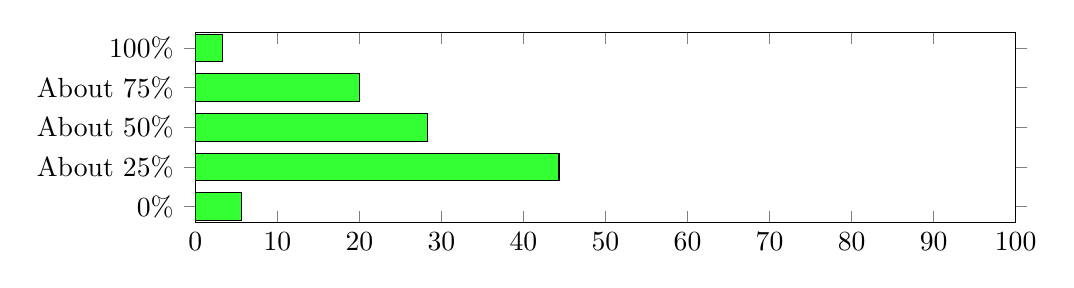
\begin{tikzpicture}
        \begin{axis}[
          xbar,
          width=12cm, 
          height=4cm, 
          bar width=10pt,
          symbolic y coords={0\%,About 25\%,About 50\%,About 75\%,100\%}, 
          ytick={0\%,About 25\%,About 50\%,About 75\%,100\%},
          xtick={0,10,...,100},
            xmin=0, xmax=100
          ]
         \addplot[fill=green!80!white] coordinates {
              (3.33,100\%) 
              (20,About 75\%) 
              (28.33,About 50\%) 
              (44.33,About 25\%) 
              (5.66,0\%)
          };
        \end{axis}
    \end{tikzpicture}
\end{boxFigure}
}


\section{Readability}

It is easy to dismiss the criticism that regex are hard to read as trivial, but in doing so, one also ignores the root cause for most of the problems they have. Their cryptic nature is not only the main contributor to errors but also the main reason why developers refrain from using regex. The following excerpt from a Vice article discussing Perl is a good representation of how regular expressions are perceived \cite{ViceProgrammingLanguagesProgrammersHate}:

{\small
\begin{quote}
    What can make Perl really look like noise is its usage of regular expressions. This is a whole other huge topic, but a regular expression is basically a way of identifying a pattern in some text or a string of text. It's a deep, weird topic and it might just result in code that looks like this:

\vspace{1cm}
\begin{minipage}{\linewidth}
\begin{verbatim}
sub deleteDoubleDots($) { 
    while($_[0] = m/\.\./) { $_[0] = s/\/[^\/]*\/\.\.//; } 
}
\end{verbatim}
\end{minipage}

… which looks a lot like Brainfuck code.
\end{quote}

}

This perception is by no means unique to the author of the article. 65\% of programmers state that they found regular expressions daunting when they first learned to code \cite{RegexesAreHard}. Part of this reaction may be caused by their complexity but most stems from the far simpler issue that they \textquote{look a lot like Brainfuck} \cite{ViceProgrammingLanguagesProgrammersHate}. The main reason for this  -- not unfounded (see listing \ref{fig:regexVsBrainfuck}) -- comparison to the infamous, esoteric programming language is the frequency of special characters which makes regex look noisy.


{
\hypersetup{citecolor=white}
\begin{listingBox}[title={Comparison of Regex \cite{regexWithComments} and Brainfuck \cite{brainfuckExample}},label=fig:regexVsBrainfuck,width=15.7cm,center]
    \textbf{Brainfuck}

\begin{lstlisting}[basicstyle=\ttfamily]
>> [>>] >> [>>]<  move to data cell
[>+>>+<<<-]>      make double copy and move to first
[[<+>-]>>[-]+<<]  restore data from one then zero second 
                      and set flag
>>                go to flag cell (0 or 1)
\end{lstlisting}

\textbf{Regex with the verbose flag}
    \begin{lstlisting}[basicstyle=\ttfamily,mathescape=true]
([a-z0-9_\.-]+)  # local Part
@                # single @ sign
([0-9a-z\.-]+)   # Domain name
\.               # single Dot .
([a-z]{2,6})$\text{\$}$     # Top level Domain
\end{lstlisting}
\end{listingBox}
}


An analysis of the 537,806 patterns from the polyglot regex corpus \cite{RegexNotLinguaFranca} shows that regular expressions contain more special characters than normal letters (see table \ref{tab:regexCharDist}). While programmers are used to a certain amount of special characters, this is a lot more than any codebase would have. For a comparison, of the $1.851.901$ characters of the gnu-core-utils codebase \cite{GnuCoreUtils} only about 20\% are special characters while 78\% are normal letters. This imbalance is not helped by the fact that, by default, regular expressions do not allow whitespaces. It comes as no suprise that 70\% of surveyed developers find regular expressions to be less readable than normal code \cite{RegexesAreHard}.

\begin{newBoxTable}[title={Character Distribution in Regex},label=tab:regexCharDist,width=11cm]{X|r|r|r}
        Character Type & Count  & \% & Mean per Pattern \\ \mytoprule
        Letters   & 8,432,429  & 42.66  & 7.97  \\ \hline
        Digits    & 1,038,590  &  5.25  & 0.98  \\ \hline
        Special Characters  & 10,296,257 & 52.09  & 9.73 \\ \hline
\end{newBoxTable}

One consequence of the high rate of special characters is that about 30\% ($317,904$) of all regexes contain escaping backslashes. This issue is well-known in the Perl community and referred to as \emph{leaning toothpick syndrome} \cite{LeaningToothpick}. 
The problem is worsened when the programming language requires backslashes in strings to be escaped themselves. In that situation, every single backslash is part of a special character in the host language like \code{"\bs n"} while double backslashes are part of the pattern \code{"\bs\bs w"}.

The syntax of regular expressions is well-suited to express concepts in the fewest characters possible but this comes with the drawback of visual noise which puts a mental burden on the reader and hides errors. It gives regex the reputation of a \enquote{write-only language} that can be understood while writing an expression but can hardly be deciphered later \cite{WriteOnlyLanguage}.


\section{Understandability}

Even when the user is able to parse the visual noise, there are still more hurdles in front of them. When the user sees a special character, correctly identifies it as unescaped and assigns it the corresponding meaning, they still cannot be completely sure if their assessment is correct. Special characters are ambiguous and their meaning is highly context-dependent which makes reading regular expressions not just hard on the eyes but on the brain as well.

For illustration let us consider the question mark \pattern{?}. Table \ref{tab:questionMark} shows seven different contexts in which the question mark means different things creating 14 different constructs in total. When a user sees a question mark they have to immediately assess the surrounding characters to find its current meaning. Does it represent itself or the optional quantifier? Does it modify a quantifier or a group? Or is it part of a look-around? 

This is no exception and applies to most special characters. The user must remember a list of rules for each special character and decide based on the surroundings which concept it represents and whether it is currently escaped. This is inherent to the compact nature of regular expressions. There are only a limited number of useable symbols and to achieve its compactness it needs to leverage not just them but also their combinations. \\

Another problem stems from the fact that how regular expressions look differs from how they work. It is easy for a user to assume that regex are a description of how the matching input looks like. Most expressions look like the expected matching input string with some parts replaced by special patterns. The pattern \pattern{".*"} from figure \ref{fig:regexSurroundingTooGreedy} seems like a correct regular expression because it has the same shape as the expected input string. The user is tempted to believe that regular expressions are a declarative language, while it is actually procedural. 

\begin{newBoxTable}[title={Ambiguity of the Question Mark Character},label=tab:questionMark,width=12cm]{X|X}
    Pattern & Meaning \\ \mytoprule
    \regex{\bs ?}, \regex{[?]} & literal question mark \\ \hline
    \regex{a?} & optional a \\ \hline
    \regex{a??, a+?, a*?, a\{X,Y\}?} & lazy quantifier \\ \hline
    \regex{(?:a)} & non-capturing group \\ \hline
    \regex{(?<name>a)} & capturing group with name \\ \hline
    \regex{a(?=b)} & positive look-ahead\\ \hline
    \regex{a(?!b)} & negative look-ahead\\ \hline
    \regex{(?<=b)a} & positive look-behind\\ \hline
    \regex{(?<!b)a} & negative look-behind\\ \hline
    \regex{(?>a+)} & atomic group \\ 
\end{newBoxTable}

In order to write correct patterns the user has to rid themselves from the notion that they describe \emph{what the input is} and think of them as sequential instructions that tell the engine \emph{how to match it}. They also have to visualize the internal state of the regex engine, otherwise they may be surprised by some of the backtracking behavior. Regex always have been intended to describe inherently procedural finite state machines but the optimization for notational convenience has given them a declarative appearance.

\section{Prone to Errors}

The issues listed above make crafting regular expressions especially error-prone. This section will give a few examples of common mistakes regex users of any experience level make. A study of 356 regex-related pull requests from 135 GitHub repositories belonging among others to Mozilla, Google, Facebook and Apache \cite{DemystifyingRegexBugs} found that regex related pull requests take longer to be merged and require more lines of code than average.

\subsection{Escaping}

The largest contributor to regex-based programming errors is the escaping of special characters. To find and avoid these mistakes the user has to know about all special characters, even the once they do not intend to use. Additionally, they must also be aware of the particular regex dialect since special characters strongly differ between them. It is also dependent on the location within the pattern since character classes automatically escape most special characters while simultaneously introducing new ones that need to be escaped instead. About 10\% of regular expression problems stem from wrong escaping \cite{DemystifyingRegexBugs}. 

\subsection{Character Classes}

Character classes are a useful and frequently used feature of regular expressions (see section \ref{sec:analysisRegexUsage}). The usage of the square brackets is reminiscent of lists in most modern programming languages which is a useful association but it can also tempt novice or absent-minded users into using a separator symbol between the single elements. This can be seen in patterns like \pattern{[0,2,3,5-9]} \cite{RegexErrorNlpChinaCharClassSep} or \pattern{[3|4|5|7|8]} \cite{RegexErrorRoncooCharClassSep} which unintentionally introduce an additional comma or pipe character into the character class. It is also important to note that most regex engines do not report a warning in these cases since duplicates in character classes are just silently removed.

\subsection{Character Ranges}

Without character ranges regex would be nearly unusable but they can be deceptive. Section \ref{sec:introAltAndCharClasses} mentions that the range \pattern{[A-z]} includes more characters than just the alphabet. Unsurprisingly this error occurs in open source codebases in different variations \cite{RegexErrorCamelLetterRange}\cite{RegexErrorApacheGeodeLetterRange}\cite{RegexErrorElasticSearchLetterRange} but is far from the only problem with character ranges.

There is an inherent disconnect between the human understanding of symbols and characters and their arrangement on the unicode table. There are plenty of character classes that contain ranges like \pattern{[\%-.]} \cite{RegexErrorJenkinsSpecialRange} and \pattern{[;-\_]} \cite{RegexErrorQuizconnectSpecialRange} that both intend to match three characters but instead match 10 and 37 respectively.

Users can also be tempted into believing that character ranges are smarter than they actually are. This manifests in character classes like \pattern{[0-31]} \cite{RegexErrorHadoopNumberRange} which showcase the expectation that character ranges have an understanding of integers which is not the case.

\section{Dialects}

Regular expressions are not only hard to read and write on their own, they are also different across languages and platforms. Although there are different standards which influenced modern regex significantly like Perl Compatible Regular Expression (PCRE) or the POSIX standard, they were not able to unify the different implementations. This does not only cause mental overhead but can also be the reason for bugs and performance problems. Given the prevalence of copied regex patterns (see figure \ref{fig:regexReuse}), it is concerning that a study found that 15\% of regular expressions show different semantics than in the language where they were taken from. Additionally, in 10\% of the cases of regex reuse the change in runtime introduced problematic performance patterns \cite{RegexNotLinguaFranca}.

About 50\% of developers believe that regex implementations can be used interchangeably \cite{RegexNotLinguaFranca}. Most regex dialects of different programming languages look fairly similar and only differ in small details. Word boundaries \pattern{\bs b} and quoting characters \pattern{\bs Q...\bs E} have special meanings in some regex dialects but are treated as normal letters in others. A developer who knows a dialect where these constructs are used may assume that they are universal. Using them in other languages can introduce bugs and unforeseen edge cases. The different dialects are yet another footgun when dealing with regular expressions -- and an unnecessary one at that. The previously mentioned study \cite{RegexNotLinguaFranca} states that:

{\small
\vspace{-1em}
\begin{quote}
    Motivated by this work, we envision a regex \enquote{universal translator} to help developers port regexes between languages.
\end{quote}
}

\noindent Alongside the readability of regex, this vision will be the primary focus of this work.

\section{Regex Denial of Service Attacks (ReDoS)} \label{sec:redos}

\begin{newBoxTable}[float=tbh,title={Visualization of Catastrophic Backtracking},label=fig:superLinear,width=13cm,halign=left]{r|cc|c|cc|c||r|cc|c|cc|c}
    & \multicolumn{2}{c|}{\bs s} & \#? & \multicolumn{2}{c|}{\bs s} & \dollar & & \multicolumn{2}{c|}{\bs s} & \#? & \multicolumn{2}{c|}{\bs s} & \dollar \\ \mytoprule
        1.  & \hly{\ws} & \hly{\ws} & \hlh{\#} & \hlg{\ws} & \hlg{\ws} & x & 10. & \hly{\ws} &      \ws  &      \#  & \hlg{\ws} & \hlg{\ws} & x \\
        2.  & \hly{\ws} & \hly{\ws} & \hlh{\#} & \hlg{\ws} &      \ws  & x & 11. & \hly{\ws} &      \ws  &      \#  & \hlg{\ws} &      \ws  & x \\
        3.  & \hly{\ws} & \hly{\ws} & \hlh{\#} &      \ws  &      \ws  & x & 12. & \hly{\ws} &      \ws  &      \#  &      \ws  &      \ws  & x \\
        4.  & \hly{\ws} & \hly{\ws} &      \#  & \hlg{\ws} & \hlg{\ws} & x & 13. &       \ws &      \ws  & \hlh{\#} & \hlg{\ws} & \hlg{\ws} & x \\
        5.  & \hly{\ws} & \hly{\ws} &      \#  & \hlg{\ws} &      \ws  & x & 14. &       \ws &      \ws  & \hlh{\#} & \hlg{\ws} &      \ws  & x \\
        6.  & \hly{\ws} & \hly{\ws} &      \#  &      \ws  &      \ws  & x & 15. &       \ws &      \ws  & \hlh{\#} &      \ws  &      \ws  & x \\
        7.  & \hly{\ws} &      \ws  & \hlh{\#} & \hlg{\ws} & \hlg{\ws} & x & 16. &       \ws &      \ws  &      \#  & \hlg{\ws} & \hlg{\ws} & x \\
        8.  & \hly{\ws} &      \ws  & \hlh{\#} & \hlg{\ws} &      \ws  & x & 17. &       \ws &      \ws  &      \#  & \hlg{\ws} &      \ws  & x \\
        9.  & \hly{\ws} &      \ws  & \hlh{\#} &      \ws  &      \ws  & x & 18. &       \ws &      \ws  &      \#  &      \ws  &      \ws  & x \\
\end{newBoxTable}



Most of the issues discussed until this point also entail security risks. Regex are commonly used for validation of user input and bugs in patterns can be exploited by malicious actors. While this is a reason for concern on its own, there is also the possibility of attackers using performance characteristics of regex patterns to amplify the effect of denial of service attacks.

The Cybersecurity \& Infrastructure Security Agency (CISA) defines a denial of service attack as following \cite{DenialOfService}:

{\small
\begin{quote}
A denial-of-service condition is accomplished by flooding the targeted host or network with traffic until the target cannot respond or simply crashes, preventing access for legitimate users. DoS attacks can cost an organization both time and money while their resources and services are inaccessible.
\end{quote}
}

Most modern regex implementations prefer NFA engines or hybrid approaches over DFA engines. The main difference is that NFA engines use backtracking and therefore allow for things like lazy quantifiers which is not possible in the non-backtracking DFA engines. More details about this topic can be found in \enquote{Mastering Regular Expressions} \cite{MasteringRegex}. This type of engine provides many benefits but can -- depending on the implementation -- also lead to the existence of so called \emph{super-linear} patterns like \pattern{\bs s*\#?\bs s*\$} which was found in Python's difflib library. When it encounters a malign input like \inp{\ws\ldots\ws\#\ws\ldots\ws x} it will backtrack $\mathcal{O}(2^n)$ times where $n$ is the sum of whitespaces on both sides of the pound sign (see figure \ref{fig:superLinear}) \cite{RedosInPractice}.

When such a pattern is present in code that is run with user-provided input -- i.e. for validation -- an attacker can pass a malign input string of arbitrary length into it. This causes the program to waste orders of magnitude more CPU time on the malicious requests than it would on regular ones. This way, super-linear patterns turn the regex engine into a force multiplier for DoS attacks.

This is not just a hypothetical threat. In 2016, a super-linear regex caused an outage of the Stackoverflow website \cite{RedosStackOverflowOutage} and exploitable regular expressions have been found in the popular Express.js framework \cite{RedosExpressJs}.

While this work does not solve the issue of ReDoS, it provides a compiler framework that translates a DSL into regex which lays the groundwork to address the problem more easily. This could take the form of compiler optimizations or linting. Even the fact that the DSL takes away some of the cognitive load associated with regular expressions could eliviate some of these security concerns.

